% **************************************************************************************************************
% A Classic Thesis Style
% An Homage to The Elements of Typographic Style
%
% Copyright (C) 2015 André Miede http://www.miede.de
%
% If you like the style then I would appreciate a postcard. My address 
% can be found in the file ClassicThesis.pdf. A collection of the 
% postcards I received so far is available online at 
% http://postcards.miede.de
%
% License:
% This program is free software; you can redistribute it and/or modify
% it under the terms of the GNU General Public License as published by
% the Free Software Foundation; either version 2 of the License, or
% (at your option) any later version.
%
% This program is distributed in the hope that it will be useful,
% but WITHOUT ANY WARRANTY; without even the implied warranty of
% MERCHANTABILITY or FITNESS FOR A PARTICULAR PURPOSE.  See the
% GNU General Public License for more details.
%
% You should have received a copy of the GNU General Public License
% along with this program; see the file COPYING.  If not, write to
% the Free Software Foundation, Inc., 59 Temple Place - Suite 330,
% Boston, MA 02111-1307, USA.
%
% **************************************************************************************************************
\RequirePackage{fix-cm} % fix some latex issues see: http://texdoc.net/texmf-dist/doc/latex/base/fixltx2e.pdf
\documentclass[ twoside,openright,titlepage,numbers=noenddot,headinclude,%1headlines,% letterpaper a4paper
                footinclude=true,cleardoublepage=empty,abstractoff, % <--- obsolete, remove (todo)
                BCOR=5mm,paper=a4,fontsize=11pt,%11pt,a4paper,%
                ngerman,american,%
                ]{scrreprt}

%********************************************************************
% Note: Make all your adjustments in here
%*******************************************************
\input{classicthesis-config}

%********************************************************************
% Bibliographies
%*******************************************************
\addbibresource{Bibliography.bib}
\addbibresource[label=ownpubs]{AMiede_Publications.bib}

%********************************************************************
% Hyphenation
%*******************************************************
%\hyphenation{put special hyphenation here}

% ********************************************************************
% GO!GO!GO! MOVE IT!
%*******************************************************
\begin{document}
\frenchspacing
\raggedbottom
\selectlanguage{spanish} % american ngerman
%\renewcommand*{\bibname}{new name}
%\setbibpreamble{}
\pagenumbering{roman}
\pagestyle{plain}
%********************************************************************
% Frontmatter
%*******************************************************
%*******************************************************
% Titlepage
%*******************************************************
\begin{titlepage}
    % if you want the titlepage to be centered, uncomment and fine-tune the line below (KOMA classes environment)
    \begin{addmargin}[-1cm]{-3cm}
    \begin{center}
        \large  

        \hfill

        \vfill

        \begingroup
            \color{Maroon}\spacedallcaps{\myTitle} \\ \bigskip
        \endgroup

        \spacedlowsmallcaps{\myName} \\
        \spacedlowsmallcaps{Asesor: \myProf}

        \vfill

        \includegraphics[width=6cm]{gfx/portada} \\ \medskip

        \mySubtitle \\ \medskip   
        %\myDegree \\
        \myDepartment \\                            
        %\myFaculty \\
        \myUni \\ \bigskip

        %\myTime\

        \vfill                      

    \end{center}  
  \end{addmargin}       
\end{titlepage}   

\pagestyle{scrheadings}
\cleardoublepage\include{FrontBackmatter/Contents}
%********************************************************************
% Mainmatter
%*******************************************************
\pagenumbering{arabic}
%\setcounter{page}{90}
% use \cleardoublepage here to avoid problems with pdfbookmark
\cleardoublepage
\section{Introducción}
En este texto hablaremos sobre qué es una curva \emph{suave} en $\realR^{2}$ y $\realR^{n}$, cómo calcular su vector tangente en cualquier punto de la curva y así determinar
su espacio tangente asociado.

Llevaremos nuestra primera definición de curva a una forma más general y veremos como calcular el espacio tangente con esta nueva definición. Para esto veremos el teorema
de la función implícita (funciones $F(x,y)=0$).

Terminaremos con una breve introdución al concepto de variedad de dimensi\'on $n$ y su espacio tangente.
\section{Justificación}
En los cursos de Cálculo se define el concepto de curva y el espacio tangente asociado a la curva. Una curva es un caso particular de un objeto más abstracto llamado subvariedad. Las subvariedades son objetos que se estudian en distintas áreas de la matemática: Topología, Análisis Matemático, Geometría Diferencial, Geometría Algebraica, etc. Es por este motivo que resulta de gran interés para cualquier estudiante de la carrera en matemáticas. En esta exposición realizamos un estudio de las subvariedades de dimensión 1 las cuales generalizan a las curvas y detallaremos la manera de calcular el espacio tangente.

\section{Objetivos}
\begin{itemize}
    \item Definir el concepto de variedad $k$-dimensional en $\realR^{n}$ y su espacio tangente asociado a un punto.
    \item Determinar la dimensi\'on de $T_{p}N$.
    \item Interpretar una curva en el plano como un caso especial de variedad utilizando el Teorema de la Funci\'on Impl\'icita.
    \item Analizar el espacio tangente de una curva como un caso particular del espacio tangente asociado a una variedad.
\end{itemize}

%*****************************************


\ctparttext{Los cuaterniones vienen de Hamilton \ldots
y han sido maldición pura para quien, de alguna forma,
los ha tocado. El vector es un sobreviviente inútil \ldots
y jamás ha sido de la más mínima utilidad para ningún ser
viviente.\\
\begin{flushright}
    \emph{Lord Kelvin}
\end{flushright}
}
\part{}
%************************************************
\chapter{Introducción}\label{ch:introduccion}
%************************************************
Cuando consideramos una función $f:\realR\mapsto\realR$, se tiene que $f$ es diferenciable en $a$ si la derivada de $f$ en $a$ existe, es decir $f'(a)$ existe. En este caso, el espacio tangente a $f$ en $a$ es una línea recta, esto es un espacio vectorial de dimensión 1. En general, si $f:\realR^{n}\mapsto\realR^{m}$, se tiene que $f$ es continua en $a$ si existe una matriz $T$ tal que

    $$\lim_{h \to 0} \| f(x+h) - f(x) - T(x) \cdot h \| = 0$$

Cuando $f$ es diferenciable, el espacio tangente está bien determinado y es un espacio vectorial de dimensión $n$.

Sin embargo cuando $f$ no es diferenciable en $a$, ¿Cómo determinamos el espacio tangente?, ¿Qué dimensión tiene?, ¿Que relación existe entre la dimensión del espacio tangente y la dimensión del espacio normal?.

Estas preguntas pueden ser extendidas a espacios mas generales como las variedades.
En el presente texto nos introduciremos al concepto de variedad y espacio tangente asociado a una variedad.


\section{Objetivos}

El objetivo de este texto es definir de manera general el concepto de superficie en $\realR^{3}$ y variedad en $\realR^{n}$.
Determinar el plano tangente de una superficie en $\realR^{3}$ (variedad en $\realR^{n}$). Determinar la dimensión del espacio tangente a una superficie (variedad) en un punto $p$. Definir el concepto de curvatura; con este estudio se darán algunos ejemplos de cálculo de curvatura y su aplicación a la Física.

\section{Justificación}

Es común ver en los estudiantes de cálculo clásico una deficiencia en el concepto de que es una superficie (variedad) y como tiene su propio cálculo diferencial estrictamente comparable con el cálculo familiar en el plano.\footnote{Mas adelante veremos como el último es consecuencia del primero.}

Esta exposición provee la noción de variedades diferenciables, la cual es indispensable en algunas ramas de las Matemáticas y sus aplicaciones basadas en el cálculo.

%*****************************************





%*****************************************
\chapter{Diferenciación}\label{ch:diferenciacion}
%*****************************************
\section{Límites y continuidad}

Esta sección está centrada en los conceptos de conjunto abierto, límite y continuidad; los conjuntos abiertos son necesarios para entender los límites y, a su vez, los límites son necesarios para entender continuidad y diferenciabilidad.

Comenzamos la formulación del concepto de conjunto abierto mediante la definición de disco abierto. Sea $x_{0}
\in  \realR^{n}$ y sea $r$ un número real positivo. El disco abierto (o bola abierta) de radio $r$ y centro 
en $x_{0}$, es el conjunto de puntos $x$ tales que $\|x-x_{0}\| < r $, como vimos el capítulo anterior. Este 
conjunto lo denotaremos por $D_{r}(x_{0})$.

\begin{definition}
    Sea $U \subset \realR^{n}$. Decimos que $U$ es un conjunto abierto cuando para cualquier punto $x_{0}$ en $U$ existe algún $r>0$
    tal que $D_{r}(x_{0})$ está contenido en $U$, es decir, $D_{r}(x_{0}) \subset U$.
\end{definition}

\begin{figure}[!ht]
  \begin{center}
      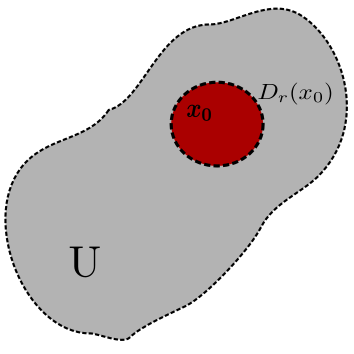
\includegraphics[width=0.5\linewidth]{gfx/conjunto-abierto}
      \caption{Un conjunto abierto $U$ es aquel que incluye completamente algún disco $D_{r}(x_{0})$ alrededor
      de cada uno de sus puntos $x_{0}$.}
      \label{fig:boat1}
  \end{center}
\end{figure}

Además establecemos la convención de que el conjunto vacio $\emptyset$ es abierto.

\begin{theorem}
    Para cada $x_{0} \in \realR^{n}$ y $r > 0$, $D_{r}(x_{0})$ es un conjunto abierto.
\end{theorem}

\begin{proof}
    Sea $x \in D_{r}(x_{0})$, esto es, sea $\|x - x_{0}\| < r$. De acuerdo con la definición
    de conjunto abierto, debemos hallar un $s > 0$ tal que $D_{s}(x) \subset  D_{r}(x_{0})$.
    Sea $s = r - \|x - x_{0}\|$, nótese que $s > 0$, pero que $s$ se hace más chico si $x$ está
    cerca del borde $D_{r}(x_{0})$ \\

    Para probar que $D_{s}(x) \subset D_{r}(x_{0})$, sea $\bm{y} \in D_{s}(x)$; esto es, sea
    $\|\bm{y} - x\| < s$. Queremos probar que también $\bm{y} \in D_{r}(x_{0})$. Probar esto en vista
    de la definición de un r-disco, equivale a demostrar que $\|\bm{y} -x_{0}\| < r$. Usemos la desigualdad
    del triángulo para esto

    \begin{eqnarray*}
        \|\bm{y} - x_{0}\| &=& \|(\bm{y} - x) + (x - x_{0})\| \\
                              &\le& \|\bm{y} - x\| + \|x - x_{0}\| \\
                              &<& s + \|x-x_{0}\| \\
                              &=& r
    \end{eqnarray*}

    De aquí que $\|\bm{y} - x_{0}\| < r$. \qed

\end{proof}

\begin{definition}
    Sea $A \subset \realR^{n}$ es punto frontera de $A$ si toda vecindad de $x$ contiene al menos un punto de $A$ y al menos un punto fuera de $A$.
\end{definition}

En esta definición, $x$ puede estar o no en $A$; si $x \in A$, entonces $x$ es un punto frontera si toda vecindad de $x$ contiene al menos un punto
que no esté en $A$. De manera análoga, si $x$ no está en $A$, es un punto frontera si toda vecindad de
$x$ contiene al menos un punto de $A$.

\begin{figure}[!ht]
  \begin{center}
      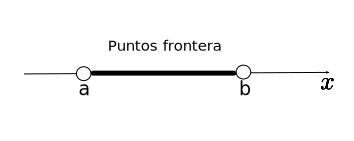
\includegraphics[width=0.5\linewidth]{gfx/puntos-frontera}
      \caption{}
      \label{fig:boat1}
  \end{center}
\end{figure}


Ya estamos en posición de definir un límite. Durante toda la exposición siguiente, el dominio de definición de la función $f$ será un conjunto abierto $A$.
Nos interesa hallar el límite de $f$ cuando $x \in A$ tienda a un punto de $A$ o a un punto frontera de $A$.

El concepto de límite es una herramienta básica y útil para el análisis de funciones; nos permite estudiar derivadas y de especial interes en este texto,
derivadas parciales.

\begin{definition}[Límite]
    Sea $f:A \subset \realR^{n} \mapsto \realR^{m}$, donde $A$ es un conjunto abierto. Sea $x_{0}$ un punto de $A$ o en la frontera de $A$, y sea
    $V$ una vecindad de $\bm{b} \in \realR^{m}$. Decimos que $f$ está en $V$ conforme $x$ tiende a $x_{0}$ si existe una vecindad $U$ de 
    $x_{0}$ tal que $x \neq x_{0}$, $x \in U$ y $x \in A$ implica $f(x) \in V$. Decimos que $f(x)$ tiende a $\bm{b}$ cuando
    $x$ tiende a $x_{0}$, es decir

    $$ \lim_{x \rightarrow x_{0}} f(x) = b $$
\end{definition}

Del cálculo de una variable sabemos que el concepto de función continua está basado en la idea intuitiva de una función cuya gráfica es una
curva sin romper, esto es, una curva sin saltos (una curva suave).

\begin{definition}
    Sea $f:A \subset \realR^{n} \mapsto \realR^{m}$ una función dada con dominio $A$. Sea $x_{0} \in A$. Decimos que $f$ es continua
    en $x_{0}$ si y sólo si
    $$ \lim_{x \rightarrow x_{0}} f(x) = f(x_{0})$$
\end{definition}

Si decimos simplemente que $f$ es \emph{continua}, queremos decir que $f$ es continua
en cada punto $x_{0}$ de $A$.

\section{Diferenciación}

En nuestro trabajo de la sección anterior vimos qué es una función continua. Aquí veremos que significa que una función sea diferenciable y como
esto nos ayuda a ver que una gráfica no esté rota, es decir, no debe haber dobleces, esquinas o picos en la gráfica. En otras palabras, la gráfica 
debe ser suave.

Para precisar estas ideas necesitamos una definición sensata de lo que entedemos por $f(x_{1}, \ldots, x_{n})$ es diferenciable en $x=(x_{1}, \ldots, x_{n})$.
En realidad esta definición no es tan sencilla, como pudiera pensarse. Necesitamos introducir el concepto de \emph{derivada parcial}. Este concepto se
basa en nuestro conocimiento del cálculo en una variable.

Entonces comenzaremos con definir que significa que $f(x)$ es diferenciable en un punto $x$, es decir, la derivada de $f(x)$ en $x$. Para esto usaremos
nuestra definición de límite.

\begin{definition}
    Sea $f$ una función de valor real definida en una vecindad abierta de $x$. Entonces $\frac{df}{dx}$ (la derivada de $f$ respecto a $x$) es
    $$ \lim_{h \rightarrow 0} \frac{f(x+h) - f(x)}{h} $$
\end{definition}

En ocasiones usaremos la notación $f'(x)$ para denotar la derivada de $f$ respecto $x$.

\begin{example}
    Sea $f(x)=x^{2}$, entonces
    \begin{eqnarray*}
        f'(3) &=& \lim_{h \rightarrow 0} \frac{f(3+h)-f(3)}{h} \\
              &=& \lim_{h \rightarrow 0} \frac{(3+h)^{2}-(3)^{2}}{h} \\
              &=& \lim_{h \rightarrow 0} (6 + h) \\
              &=& 6
    \end{eqnarray*}
    Entonces $f'(3) = 6$.
\end{example}

\begin{figure}[!ht]
  \begin{center}
      \includegraphics[width=0.5\linewidth]{gfx/derivative-example}
      \caption{$f(x)=x^{2}$}
      \label{fig:boat1}
  \end{center}
\end{figure}

De forma geométrica, la derivada nos dice la \emph{pendiente} de la recta tangente a $f$ en un punto $x$.

Que una función $f(x)$ sea diferenciable en todo su dominio quiere decir que para cualquier $x$ en el dominio de $f(x)$ existe
$f'(x)$, esto nos dice que la gráfica de $f(x)$ es suave. Esto nos acerca a la definición de \emph{curva}. Un ejemplo típico 
de una gráfica no suave la vemos en el siguiente ejemplo

\begin{myExample}
    Sea $f(x) = |x|$ con $f:\realR \rightarrow \realR^{2}$, vemos que la derivada en $x=0$ no existe.
    \begin{eqnarray*}
        f'(0) &=& \lim_{h \rightarrow 0} \frac{f(h) - f(0)}{h} \\
              &=& \lim_{h \rightarrow 0} \frac{0}{0}
    \end{eqnarray*}
\end{myExample}

\begin{figure}[!ht]
  \begin{center}
      \includegraphics[width=0.6\linewidth]{gfx/grafica-abs}
      \caption{gráfica no suave}
      \label{fig:boat1}
  \end{center}
\end{figure}

Transportando esta idea a funciones de varias variables surge la definición de \emph{derivada parcial}.

\begin{definition}
    Sean $U \subset \realR^{n}$ un conjunto abierto y $f:U \subset \realR^{n} \rightarrow \realR$ una función con valores reales. Entonces $\partial f/\partial x_{1},
    \ldots, \partial f/ \partial x_{n}$, las derivadas parciales de $f$ respecto a la primera, segunda, \dots, n-ésima variable son las funciones con valores
    reales, de $n$ variables, las cuales, en el punto $(x_{1},\ldots,x_{n}) = x$, están definidas por
    \begin{eqnarray*}
        \frac{\partial f}{\partial x_{j}} (x_{1},\ldots,x_{n}) &=& \lim_{h \rightarrow 0} \frac{f(x_{1},x_{2},\ldots,x_{j} + h,\ldots,x_{n}) - f(x_{1},\ldots,x_{n})}{h} \\
                                                               &=& \lim_{h \rightarrow 0} \frac{f(x+he_{j})-f(x)}{h} 
    \end{eqnarray*}
    si existen los límites, donde $1 \le j \le n$ y $e_{j}$ es el j-ésimo vector de la base canónica.
\end{definition}

En otras palabras, $\partial f / \partial x_{j}$ es simplemente la derivada de $f$ respecto a la variable $x_{j}$, manteniendo las otras variables fijas.

\begin{myExample}
    Si $f(x,y) = x^{2}y+y^{3}$, hallar $\partial f / \partial x$ y $\partial f / \partial y$.
    Para hallar $\partial f / \partial x$ mantenemos $y$ constante y diferenciamos sólo respecto de $x$, entonces
    $$ \frac{\partial f}{\partial x} = \frac{d(x^{2}y+y^{3})}{dx} = 2xy $$

    De forma análoga, tenemos que
    $$ \frac{\partial f}{\partial y} = \frac{d(x^{2}y+y^{3})}{dy} = x^{2} + 3y^{2} $$
\end{myExample}
%*****************************************
%*****************************************
%*****************************************
%*****************************************
%*****************************************


\ctparttext{Yo me alejo con espanto y horror, de la triste
maldad de las funciones que no tienen derivadas.\\
\begin{flushright}
    \emph{Charles Hermite}
\end{flushright}
}
\part{}
\chapter{Curvas en $\realR^{3}$}\label{ch:curvas-en-r3}

En este capítulo daremos una primera definición de \emph{curva}, con la cual trabajaremos
a lo largo de esta sección. En el siguiente capítulo daremos una definición más general.
Veremos como calcular el vector tangente a la curva y como encontrar su espacio tangente.

Es importante mencionar que aunque nuestros casos serán para $\realR^{3}$ son totalmente
válidos para $\realR^{2}$.

\section{¿Qu\'e es una curva?}

Si nos pidieran dar un ejemplo de una curva, podriamos decir que una l\'inea recta, como
$y-2x=1$ (aunque no sea \emph{curva}), o un c\'irculo, por ejemplo $x^{2} + y^{2} = 1$, 
o tal vez una par\'abola, $y-x^{2}=0$.

Todas estas curvas est\'an descritas por su ecuaci\'on cartesiana
$$ f(x,y) = c \text{,} $$
donde $f$ es una funci\'on de $x$ y $y$ y $c$ es constante. Todos estos ejemplos son curvas
en $\realR^{2}$, pero podr\'iamos considerar curvas en $\realR^{3}$ tambi\'en, por ejemplo
el eje $x$ en $\realR^{3}$ es la l\'inea recta dada por
$$y=0\text{,} \quad z=0 \text{,}$$
y de forma general una curva en $\realR^{3}$ se puede definir con el par de ecuaciones
$$ f(x,y,z)=c_{1}\text{,}\quad f(x,y,z)=c_{2} \text{,}$$
curvas de \'este estilo son llamadas \emph{curvas de nivel}.

Pero existe una forma diferente de pensar las curvas que nos ayudar\'a en muchas ocasiones.
Podemos ver a una curva como la trayectoria recorrida por un punto en movimiento. As\'i
$c(t)$, es la posici\'on del punto en el tiempo $t$. Usaremos esta idea para dar nuestra
primera definici\'on formal de curva en $\realR^{3}$

\begin{definition}
    Una curva parametrizada en $\realR^{3}$ es una mapeo $c:(\alpha,\beta) \rightarrow \realR^{3}$,
    para alg\'un $\alpha$, $\beta$ con $-\infty \le \alpha < \beta \le \infty$.
\end{definition}

\begin{myExample}
    Una línea recta es el tipo más simple de \emph{curva} en el espacio Euclideo. Es una curva
    $c:\realR \rightarrow \realR^{3}$ tal que
    $$ c(t) = p + tq$$
    Donde $p$,$q$ $\in \realR^{3}$
\end{myExample}

\begin{myExample}
    La curva (hélice) $t \rightarrow (a\cos{t},a\sin{t},0)$ viaja alrededor de un círculo de 
    $a > 0$ en el plano $xy$ de $\realR^{3}$. Si dejamos que la curva suba a baje de manera
    uniforme, obtenemos la hélice $c:\realR \rightarrow \realR^{3}$, dada por
    $$ c(t) = (a\cos{t}, a\sin{t}, bt) $$
    donde $a>0$, $b \ne 0$
\end{myExample}

\begin{figure}[!ht]
  \begin{center}
      \includegraphics[width=0.6\linewidth]{gfx/helice}
      \caption{Hélice}
      \label{fig:boat1}
  \end{center}
\end{figure}

Estas curvas estar\'an descritas exclusivamente en t\'erminos de funciones \emph{suaves}: una funci\'on
$f:(\alpha,\beta) \rightarrow \realR$ se dice que es \emph{suave} si sus derivadas $\frac{d^{n}f}{dt^{n}}$
existen para todo $n \ge 1$.

Para diferenciar una \emph{funci\'on vectorial} como $c(t)$, diferenciamos componente a componente, si
$$ c(t) = (c_{1}(t),c_{2}(t),c_{3}(t))\text{,}$$
entonces
$$ \frac{dc}{dt} = \left( \frac{dc_{1}}{dt},\frac{dc_{2}}{dt},\frac{dc_{3}}{dt}\right)\text{.}$$

De aqu\'i en adelante todas las curvas parametrizadas en este texto se asumiran suaves.

\section{Vector tangente a una curva parametrizada}

\begin{definition}
    Si $c$ es una curva parametrizada, su primera derivada $c'(t)$ es llamada el vector tangente
    de $c$ en el punto $c(t)$.
\end{definition}

\begin{myExample}
    El caracol de Pascal es la curva parametrizada
    $$ c(t)=((1+2\cos{t})\cos{t},(1+2\cos{t}+2\cos{t})\text{,} \quad t \in \realR$$
    El vector tangente es
    $$ c'(t)=(-\sin{t}-2\sin{2t},\cos{t}+2\cos{2t})$$
    En particular,
    $$ c'(2\pi/3) = (\sqrt{3}/2,-3/2)$$
\end{myExample}

\begin{figure}[!ht]
  \begin{center}
      \includegraphics[width=0.7\linewidth]{gfx/limacon2}
      \caption{Curva de Pascal}
      \label{fig:boat1}
  \end{center}
\end{figure}


Esta definición puede ser interpretada geometricamente de la siguiente forma. La derivada en
$t$ de la función de valor real $f$ en $\realR$ esta dada por

$$ \frac{df}{dt}(t) = \lim_{h \rightarrow 0} \frac{f(t+h)-f(t)}{h} $$

Esta expresión también tiene sentido si remplazamos $f$ por una curva $c = (c_{1},c_{2},c_{3})$,
es decir,

$$ \frac{1}{h}(c(t+h)-c(t)) =$$
$$\left( \frac{c_{1}(t+h)-c_{1}(t)}{h},\frac{c_{2}(t+h)-c_{2}(t)}{h},\frac{c_{3}(t+h)-c_{3}(t)}{h} \right) $$

Este es el vector $c(t)$ hacia $c(t+h)$, multiplicado escalarmente por $\frac{1}{h}$. Ahora, cuando $h$ se hace
muy pequeño, $c(t+h)$ se aproxima a $c(t)$ y en el límite $h \rightarrow 0$, obtenemos el vector tangente
$$\left( \frac{dc_{1}}{dt}(t),\frac{dc_{2}}{dt}(t),\frac{dc_{3}}{dt}(t) \right) $$
el cual tiene como punto inicial $c(t)$.

\section{Espacio tangente a una curva parametrizada}

Sabemos que dados un punto $p$ y una direcci\'on $u$ podemos describir parametricamente una
l\'inea recta que contenga a $p$ con direcci\'on de $u$ (paralela a $u$) de la forma
$$ l(t) = p + tu \text{,} \quad t \in \realR \text{.}$$

Tomaremos esta idea para definir el \emph{espacio tangente} a una curva.

\begin{definition}
    Si $c(t)$ es una curva parametrizada, entonces el espacio tangente (recta tangente) a $c(t)$ es
    $$ l(t_{1}) = ( c(t) + t_{1}c'(t) ) \text{,} \quad t_{1} \in \realR \text{.}$$
\end{definition}

\begin{myExample}
    Tomando el ejemplo 3.4, el espacio tangente (recta tangente) en $c(\pi/4)$ es
    $$ l(t_{1}) = (c(\pi/4) + t_{1}c'(\pi/4)) $$
\end{myExample}

\begin{figure}[!ht]
  \begin{center}
      \includegraphics[width=0.8\linewidth]{gfx/limacon}
      \caption{Espacio tangente a la curva de Pascal $c$ en $c(\pi/4)$}
      \label{fig:boat1}
  \end{center}
\end{figure}



%\addtocontents{toc}{\protect\clearpage} % <--- just debug stuff, ignore
%\chapter{Curvas en $\realR^{3}$}\label{ch:curvas-en-r3}

En este capítulo daremos una primera definición de \emph{curva}, con la cual trabajaremos
a lo largo de esta sección. En el siguiente capítulo daremos una definición más general.
Veremos como calcular el vector tangente a la curva y como encontrar su espacio tangente.

Es importante mencionar que aunque nuestros casos serán para $\realR^{3}$ son totalmente
válidos para $\realR^{2}$.

\section{¿Qu\'e es una curva?}

Si nos pidieran dar un ejemplo de una curva, podriamos decir que una l\'inea recta, como
$y-2x=1$ (aunque no sea \emph{curva}), o un c\'irculo, por ejemplo $x^{2} + y^{2} = 1$, 
o tal vez una par\'abola, $y-x^{2}=0$.

Todas estas curvas est\'an descritas por su ecuaci\'on cartesiana
$$ f(x,y) = c \text{,} $$
donde $f$ es una funci\'on de $x$ y $y$ y $c$ es constante. Todos estos ejemplos son curvas
en $\realR^{2}$, pero podr\'iamos considerar curvas en $\realR^{3}$ tambi\'en, por ejemplo
el eje $x$ en $\realR^{3}$ es la l\'inea recta dada por
$$y=0\text{,} \quad z=0 \text{,}$$
y de forma general una curva en $\realR^{3}$ se puede definir con el par de ecuaciones
$$ f(x,y,z)=c_{1}\text{,}\quad f(x,y,z)=c_{2} \text{,}$$
curvas de \'este estilo son llamadas \emph{curvas de nivel}.

Pero existe una forma diferente de pensar las curvas que nos ayudar\'a en muchas ocasiones.
Podemos ver a una curva como la trayectoria recorrida por un punto en movimiento. As\'i
$c(t)$, es la posici\'on del punto en el tiempo $t$. Usaremos esta idea para dar nuestra
primera definici\'on formal de curva en $\realR^{3}$

\begin{definition}
    Una curva parametrizada en $\realR^{3}$ es una mapeo $c:(\alpha,\beta) \rightarrow \realR^{3}$,
    para alg\'un $\alpha$, $\beta$ con $-\infty \le \alpha < \beta \le \infty$.
\end{definition}

\begin{myExample}
    Una línea recta es el tipo más simple de \emph{curva} en el espacio Euclideo. Es una curva
    $c:\realR \rightarrow \realR^{3}$ tal que
    $$ c(t) = p + tq$$
    Donde $p$,$q$ $\in \realR^{3}$
\end{myExample}

\begin{myExample}
    La curva (hélice) $t \rightarrow (a\cos{t},a\sin{t},0)$ viaja alrededor de un círculo de 
    $a > 0$ en el plano $xy$ de $\realR^{3}$. Si dejamos que la curva suba a baje de manera
    uniforme, obtenemos la hélice $c:\realR \rightarrow \realR^{3}$, dada por
    $$ c(t) = (a\cos{t}, a\sin{t}, bt) $$
    donde $a>0$, $b \ne 0$
\end{myExample}

\begin{figure}[!ht]
  \begin{center}
      \includegraphics[width=0.6\linewidth]{gfx/helice}
      \caption{Hélice}
      \label{fig:boat1}
  \end{center}
\end{figure}

Estas curvas estar\'an descritas exclusivamente en t\'erminos de funciones \emph{suaves}: una funci\'on
$f:(\alpha,\beta) \rightarrow \realR$ se dice que es \emph{suave} si sus derivadas $\frac{d^{n}f}{dt^{n}}$
existen para todo $n \ge 1$.

Para diferenciar una \emph{funci\'on vectorial} como $c(t)$, diferenciamos componente a componente, si
$$ c(t) = (c_{1}(t),c_{2}(t),c_{3}(t))\text{,}$$
entonces
$$ \frac{dc}{dt} = \left( \frac{dc_{1}}{dt},\frac{dc_{2}}{dt},\frac{dc_{3}}{dt}\right)\text{.}$$

De aqu\'i en adelante todas las curvas parametrizadas en este texto se asumiran suaves.

\section{Vector tangente a una curva parametrizada}

\begin{definition}
    Si $c$ es una curva parametrizada, su primera derivada $c'(t)$ es llamada el vector tangente
    de $c$ en el punto $c(t)$.
\end{definition}

\begin{myExample}
    El caracol de Pascal es la curva parametrizada
    $$ c(t)=((1+2\cos{t})\cos{t},(1+2\cos{t}+2\cos{t})\text{,} \quad t \in \realR$$
    El vector tangente es
    $$ c'(t)=(-\sin{t}-2\sin{2t},\cos{t}+2\cos{2t})$$
    En particular,
    $$ c'(2\pi/3) = (\sqrt{3}/2,-3/2)$$
\end{myExample}

\begin{figure}[!ht]
  \begin{center}
      \includegraphics[width=0.7\linewidth]{gfx/limacon2}
      \caption{Curva de Pascal}
      \label{fig:boat1}
  \end{center}
\end{figure}


Esta definición puede ser interpretada geometricamente de la siguiente forma. La derivada en
$t$ de la función de valor real $f$ en $\realR$ esta dada por

$$ \frac{df}{dt}(t) = \lim_{h \rightarrow 0} \frac{f(t+h)-f(t)}{h} $$

Esta expresión también tiene sentido si remplazamos $f$ por una curva $c = (c_{1},c_{2},c_{3})$,
es decir,

$$ \frac{1}{h}(c(t+h)-c(t)) =$$
$$\left( \frac{c_{1}(t+h)-c_{1}(t)}{h},\frac{c_{2}(t+h)-c_{2}(t)}{h},\frac{c_{3}(t+h)-c_{3}(t)}{h} \right) $$

Este es el vector $c(t)$ hacia $c(t+h)$, multiplicado escalarmente por $\frac{1}{h}$. Ahora, cuando $h$ se hace
muy pequeño, $c(t+h)$ se aproxima a $c(t)$ y en el límite $h \rightarrow 0$, obtenemos el vector tangente
$$\left( \frac{dc_{1}}{dt}(t),\frac{dc_{2}}{dt}(t),\frac{dc_{3}}{dt}(t) \right) $$
el cual tiene como punto inicial $c(t)$.

\section{Espacio tangente a una curva parametrizada}

Sabemos que dados un punto $p$ y una direcci\'on $u$ podemos describir parametricamente una
l\'inea recta que contenga a $p$ con direcci\'on de $u$ (paralela a $u$) de la forma
$$ l(t) = p + tu \text{,} \quad t \in \realR \text{.}$$

Tomaremos esta idea para definir el \emph{espacio tangente} a una curva.

\begin{definition}
    Si $c(t)$ es una curva parametrizada, entonces el espacio tangente (recta tangente) a $c(t)$ es
    $$ l(t_{1}) = ( c(t) + t_{1}c'(t) ) \text{,} \quad t_{1} \in \realR \text{.}$$
\end{definition}

\begin{myExample}
    Tomando el ejemplo 3.4, el espacio tangente (recta tangente) en $c(\pi/4)$ es
    $$ l(t_{1}) = (c(\pi/4) + t_{1}c'(\pi/4)) $$
\end{myExample}

\begin{figure}[!ht]
  \begin{center}
      \includegraphics[width=0.8\linewidth]{gfx/limacon}
      \caption{Espacio tangente a la curva de Pascal $c$ en $c(\pi/4)$}
      \label{fig:boat1}
  \end{center}
\end{figure}



%\include{multiToC} % <--- just debug stuff, ignore for your documents
% ********************************************************************
% Backmatter
%*******************************************************
\appendix
%\renewcommand{\thechapter}{\alph{chapter}}
\cleardoublepage
\ctparttext{Algunos trucos de cálculo son bastante fáciles,
otros son muy difíciles. Los que escriben los libros de matemáticas
avanzadas pocas veces se toman la molestia de mostrar cuán fáciles
son los cálculos fáciles.\\
\begin{flushright}
    \emph{Silvanus P. Thompson, Calculus Made Easy (1910)}
\end{flushright}
}


\part{Appendix}
%********************************************************************
% Appendix
%*******************************************************
% If problems with the headers: get headings in appendix etc. right
%\markboth{\spacedlowsmallcaps{Appendix}}{\spacedlowsmallcaps{Appendix}}
\chapter{Algunas definiciones \'utiles}

\begin{definition}[Morfismo]
    \label{def:morphism}
    Es un mapeo que conserva la estructura de un objeto matem\'atico a otro. En este texto, vemos a los
    morfismos como funciones cuando van de conjunto a conjunto, y como transformaciones lineales cuando
    se define entre espacios vectoriales.
\end{definition}

\begin{definition}[Isomorfismo]
    \label{def:isomorphism}
    Es un morfismo que admite una inversa.
\end{definition}

\begin{theorem}
    Dos espacios vectoriales son isomorfos si y solo si tienen la misma dimensi\'on.
\end{theorem}

\begin{lemma}
    \label{lem:vector-space-dimension}
    Si dos espacios vectorial son isomorfos entonces tienen la misma dimensi\'on.
\end{lemma}

\begin{definition}[Difeomorfismo]
    \label{def:diffeomorphism}
    Es un isomorfismo diferenciable. Su inversa tambi\'en es diferenciable.
\end{definition}



\section{Bibliografia}
\begin{itemize}
\item Jerrold E. Marsden, A. J. T. (1991). Cálculo Vectorial. Addison-Wesley. 

\item Lang, S. (1970). Introducction to Linear Algebra. Springer. 

\item Thompson, S. P. (1910). Calculus Made Easy. The Macmillan Company. 

\item MacTutor, (2016, Septiembre 26), http://www-history.mcs.st-andrews.ac.uk/Biographies/Hamilton.html
\item MacTutor, (2016, Septiembre 26), http://www-history.mcs.st-andrews.ac.uk/Biographies/Grassmann.html
\item MacTutor, (2016, Septiembre 26), http://www-history.mcs.st-andrews.ac.uk/Biographies/Gibbs.html
\end{itemize}

%********************************************************************
% Other Stuff in the Back
%*******************************************************
%\cleardoublepage
\section{Bibliografia}
\begin{itemize}
\item Jerrold E. Marsden, A. J. T. (1991). Cálculo Vectorial. Addison-Wesley. 

\item Lang, S. (1970). Introducction to Linear Algebra. Springer. 

\item Thompson, S. P. (1910). Calculus Made Easy. The Macmillan Company. 

\item MacTutor, (2016, Septiembre 26), http://www-history.mcs.st-andrews.ac.uk/Biographies/Hamilton.html
\item MacTutor, (2016, Septiembre 26), http://www-history.mcs.st-andrews.ac.uk/Biographies/Grassmann.html
\item MacTutor, (2016, Septiembre 26), http://www-history.mcs.st-andrews.ac.uk/Biographies/Gibbs.html
\end{itemize}

%\cleardoublepage\include{FrontBackmatter/Declaration}
%\cleardoublepage\include{FrontBackmatter/Colophon}
% ********************************************************************
% Game Over: Restore, Restart, or Quit?
%*******************************************************
\end{document}
% ********************************************************************
